\documentclass[a4paper]{article}
\usepackage[utf8]{inputenc}
\usepackage[a4paper, margin=1in]{geometry}
\usepackage{enumitem}
\usepackage{pgfplots}
\usepackage{amsmath}
\usepackage{hyperref}
\usepackage{listings}
\usepackage{tabularx}
\usepackage{xcolor}
\usepackage[super]{nth}

\pgfplotsset{compat=1.16}
\renewcommand{\arraystretch}{1.5}

\definecolor{codegreen}{rgb}{0,0.6,0}
\definecolor{codegray}{rgb}{0.5,0.5,0.5}
\definecolor{codepurple}{rgb}{0.58,0,0.82}
\definecolor{backcolour}{rgb}{0.95,0.95,0.92}

\lstdefinestyle{mystyle}{
    backgroundcolor=\color{backcolour},   
    commentstyle=\color{codegreen},
    keywordstyle=\color{magenta},
    numberstyle=\tiny\color{codegray},
    stringstyle=\color{codepurple},
    basicstyle=\ttfamily\footnotesize,
    breakatwhitespace=false,         
    breaklines=true,                 
    captionpos=b,                    
    keepspaces=true,                 
    numbers=left,                    
    numbersep=5pt,                  
    showspaces=false,                
    showstringspaces=false,
    showtabs=false,                  
    tabsize=2
}
\lstset{style=mystyle}

\title{ASL Assignment 4}
\author{Fabian Wüthrich}

\begin{document}

\maketitle

\begin{enumerate}
    \item Cache Mechanics (40 pts)
        \begin{enumerate}
            \item 
                \textbf{Cache Misses} \verb|calculate1| \vspace{1mm} 

                  The vector $v$ has a size of 8448 bytes and doesn't fit in
                  cache completely. This implies that for every row of $A$ we
                  have to load $v$ into cache again. 

                  The elements \verb|v[j]| and \verb|A[i * m + j]| are 8448
                  bytes apart in memory so they are assigned to different sets
                  in cache. Therefore, the block of \verb|v| and the block of
                  \verb|A| will not interfere with each other. Every \nth{16}
                  iteration we have a miss for the first \verb|v[j]| and
                  \verb|A[i * m + j]|. The second access to \verb|v[j]| is not
                  a miss, as the value was loaded before. In total, there are
                  $\frac{2mn}{16}=\frac{mn}{8}$ misses and we access \verb|v|
                  and \verb|A| $3nm$ times. The miss rate is then
                  $\frac{1}{24} \approx 0.042$.
                  \vspace{1mm}

                  \textbf{Cache Misses} \verb|calculate2| \vspace{1mm}

                  In the inner loop \verb|v[j]| get loaded
                  once and is then reused $n$ times. There is a potential
                  conflict with \verb|A[(i + n - 1) * m + j]| as this value is
                  mapped to the same set. As we have a 2-way set associative
                  cache with LRU replacement, this conflict is resolved by
                  leaving \verb|v[i]| in the first block (as it was used in the
                  previous loop) and replace \verb|A[(i + n - 1) * m + (j - 1)]| 
                  (placed in the second block in the previous iteration). This 
                  gives us a compulsory miss in every \nth{16} iteration so we
                  have $\frac{m}{16}$ misses for $v$.

                  The values of $A$ get mapped to different sets (each value is
                  placed 4 sets apart from the set of the previous value) so
                  there will be no conflicts between values of $A$. In every
                  \nth{16} iteration we have $n$ compulsory misses followed by
                  a series of cache hits. Thus, there are
                  $\frac{nm}{16}$ misses for $A$ which gives
                  $\frac{m+mn}{16}$ total misses.

                  The number of accesses is the same as above so we get a cache
                  miss rate of
                  
                  \begin{equation*}
                      \frac{m+nm}{16} \cdot \frac{1}{3mn} = \frac{n+1}{48n}
                      = \frac{3}{128} \approx 0.023
                  \end{equation*}

                  which is better than \verb|calculate1|.
              \item 
                \textbf{Cache Misses} \verb|calculate1| \vspace{1mm} 

                As $n$ doesn't influence the cache access pattern of
                \verb|calculate1|, the miss rate is still
                $\frac{1}{24}$.
                \vspace{1mm}

                \textbf{Cache Misses} \verb|calculate2| \vspace{1mm} 

                Due to the LRU policy $v$ stays in cache as before so the miss
                rate is still $\frac{m}{16}$. 

                For $A$ we get a new conflict as
                \verb|A[(i + 8) * m + j]| is mapped to the same set as
                \verb|A[i * m + j]|. This conflict is again resolve by putting 
                \verb|A[(i + 8) * m + j]| in the other block of the set. In the 
                next iteration we a hit for both \verb|A[i * m + (j + 1)]| and 
                \verb|A[(i + 8)  * m + (j + 1)]| as they were loaded with the
                previous line.

                A problem occurs when we get to the set that contains $v$. In
                this case one block is already occupied by \verb|v[j]| and we
                have to kick out the value of $A$ stored in the other block.
                This causes two misses in every inner loop iteration plus the
                additional $n-2$ misses in every \nth{16} outer loop iteration. 
                Thus, we have $2m+(n-2)\frac{m}{16}$ misses for $A$.

                Adding everything together gives us $\frac{mn+31m}{16}$ cache
                misses and a cache miss rate of
                \begin{equation*}
                    \frac{mn+31m}{16} \cdot \frac{1}{3mn} = \frac{n+31}{48n}
                    = \frac{47}{768} \approx 0.061
                \end{equation*}
            \item When $n=16$ we observed a conflict miss in the set where
                $v$ is stored. If we increase $n$ further, we can see that we get more
                conflict misses (e.g. \texttt{A[0 * m + j]} and 
                \texttt{A[16 * m + j]} get mapped to the same set which causes
                a conflict miss in the next outer loop iteration) and the miss
                rate increases.

                Now if we set $n=23$ we produce conflict misses for 
                \texttt{A[0 * m + j]} \dots \texttt{A[7 * m + j]} which get
                removed from cache. We have to load these values again in the
                next outer loop iteration and because of the LRU policy we
                overwrite \texttt{A[8 * m + j]} \dots \texttt{A[15 * m + j]}.
                
                The pattern continues like that so in the end we have only
                misses for $A$. Increasing $n$ is not necessary as 
                \texttt{A[7 * m + j]} falls into the same set as $v$, so was
                already replaced in a previous iteration of the inner loop.
                A smaller $n$ gives a lower cache rate because there would be
                still values of $A$ left in the cache, which gives a hit in the
                next outer loop iteration. Therefore, $n=23$ is the minimum
                value that produces the highest miss rate.

            \item The problem in the previous subtask was that
                \texttt{calculate2} does not use the full cache block before it
                goes to the next row. Thus, the block is not in cache anymore
                if we want to access it in the next outer loop iteration.

                We can fix this with blocking as seen in the lecture, so we traverse 
                $A$ in $n \times 16$ blocks. The following listing shows the
                improvement.
                \begin{lstlisting}[language=C]
void  calculate2(float *A, float* v, int m, int n) {
  for (int j = 0; j < m; j += 16) {
    for (int i = 0; i < n; ++i) {
      for (int k = 0; k < 16; ++k) {
        v[j + k] = max(v[j + k], A[i * m + j + k]);
      }
    }
  }
}
\end{lstlisting}
               With this improvement we use the complete cache block in the
               inner most loop and then we do not use these values again, so we
               will not get any conflict misses as in the previous subtask.

               For $v$ we get again the $\frac{m}{16}$ compulsory misses. For
               $A$ we get a in every outer loop iteration one cache miss per
               row i.e. $\frac{m}{16} \cdot n$. Thus, we have
               $\frac{m+mn}{16}$ misses in total and a cache miss rate of
               \begin{equation*}
                   \frac{m+mn}{16} \cdot \frac{1}{3mn} = \frac{n+1}{48n}
                   = \frac{1}{46} \approx 0.022
               \end{equation*}
               As $n$ doesn't influence the cache miss rate of
               \texttt{calculate1}, the function has still a miss rate of
               $0.042$ which is inferior to the improvement of
               \texttt{calculate2}.
        \end{enumerate}
    \item Stride Access (20 pts)
\begin{enumerate}
    \item The function \verb|calculate| accesses $v$ twice with $stride=4$. In
        the first iteration of the outer loop we get a hit in every second
        iteration of the inner loop (one cache block can hold 8 doubles). We
        cannot improve the number of hits in the first round by adjusting
        $n$ because of the compulsory misses. Now we have to pick $n$ such that
        every element of $v$ is still in the cache if we access $v$ in the
        second iteration and we have only hits. The whole cache can hold 512 double values so if we
        choose $n$ to access more values we get conflicts and more misses in
        the second iteration of the outer loop. Thus, the maximum value is
        $n=128$ which loads the value at index 508 as last element into the
        cache.

    \item As in the previous answer we cannot influence the misses in the first
        outer loop iteration by adjusting $n$. In order to generate more misses
        in the second iteration we fill the cache with 768 doubles which
        overrides the first 256 doubles of $v$ in the cache. In the second iteration
        we have to load the first 256 doubles again and this will overwrite the
        next 256 doubles that where in cache (LRU policy). Then we load the
        second portion and this removes the last chunk of 256 doubles from the
        cache. Now we get a miss
        in every second iteration in the second round which is the lowest hit
        rate we can achieve. Therefore, the minimum value to get the lowest hit rate is
        $n=192$.

    \item Now we have $stride = 32$ which forces a compulsory miss in every
        iteration in the first round. In order to create only hits in the
        second round (highest hit rate) we have to set $n=16$ which access the 
        value at index 480 and doesn't generate any conflicts with the previous 
        sets.

        For the lowest hit rate we set $n=24$ which is the minimum value to
        load 768 doubles so we remove the values in a equally bad way as in the
        previous sub-task. Now we have only misses for both outer loop
        iterations which is the lowest hit rate we can achieve.
    
    \item With $stride=16$ every two consecutive values we access are 128 bytes apart.
        This is too large to fit into a block of 64 bytes and we do not have
        spatial locality. Because of that we
        have just compulsory misses in the first round and no hit at all.

        As $n=40$ we load 640 doubles which is with 5120 bytes too
        large to fit in cache. The cache can hold 512 doubles so the first 128
    doubles (\texttt{v[0]}\dots\texttt{v[127]}) get overwritten by the last 128
    doubles (\texttt{v[512]}\dots\texttt{v[639]}) of $v$ in the first round. 

        In the second iteration we get conflicts at the 16 sets in the
        beginning because the required values were overwritten in the first
        iteration. When we consider the LRU policy one can see that we have
        only misses for the first 16 sets because the values overwrite each
        other.

        The last 16 sets of the cache generate now conflicts so we can reuse the
        256 doubles which we placed there in the first iteration. With a stride
        of 16 we achieve 16 hits on these 256 doubles.

        We access $v$ 80 times so we get a hit rate of $\frac{16}{80} \approx
        0.2$.

        For completeness I summarize the hit/miss pattern for the whole
        calculation. In the first outer loop iteration we have 40 compulsory
        misses. Then when we traverse $v$ a second time we have 8 misses,
        8 hits, 8 misses, 8 hits and again 8 misses in the end.
       \end{enumerate}
    \item Rooflines (40 pts)
        \begin{enumerate}
            \item Without SIMD instructions we can perform one FMA instruction
                on P0, one FMA instruction on P1 and one addition on P2. As an
                FMA instruction executes two floating point instructions per
                cycle we get a peak performance of $\pi_1 = 2 + 2 + 1 = 5 \,
                flops/cycle$.

                With SIMD instructions enabled we can use the previous
                instructions on vector of four doubles which gives a peak 
                performance of $\pi_2 = 8 + 8 + 4 = 20 \, flops/cycle$.

                The given computer has a maximum read bandwidth of $\beta = 32 \,
                bytes/cycle$ which is the same for the model with SIMD and the
                one without.

                Using the peak performance and the maximum read bandwidth we
                can plot the following roofline models.

                \begin{center}
                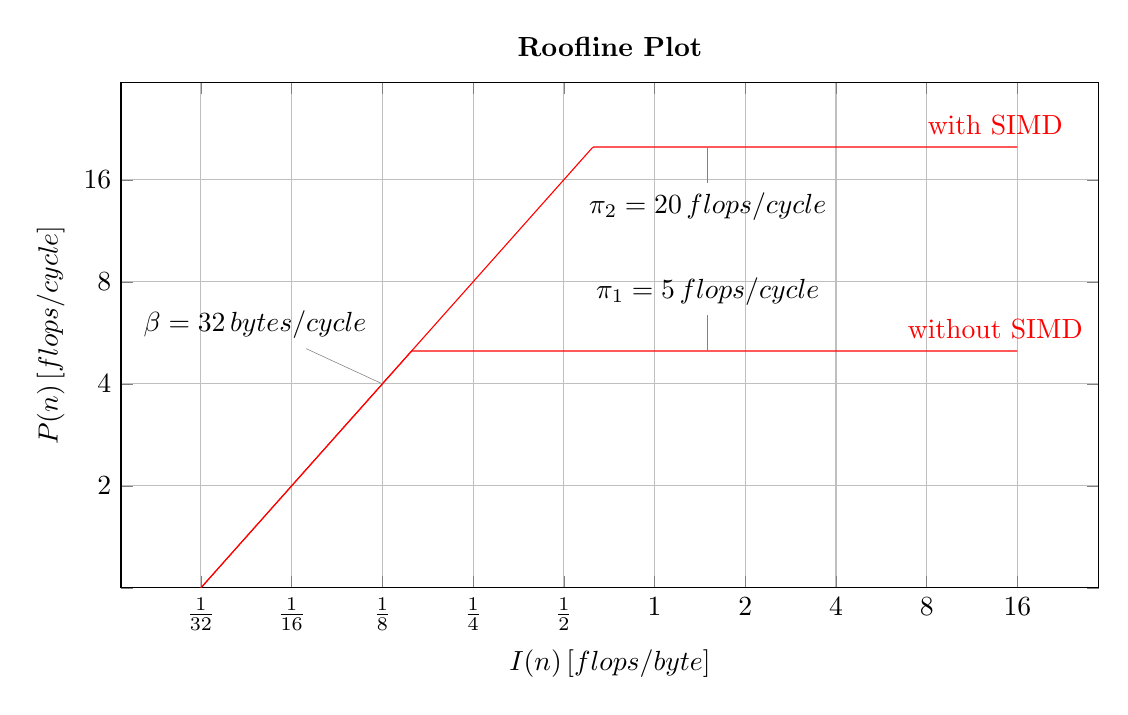
\begin{tikzpicture}
                    \begin{axis}[
                            title=\textbf{Roofline Plot},
                            width=14cm,
                            height=8cm,
                            xmode=log,
                            xlabel={$I(n) \, [flops/byte]$},
                            log basis x={2},
                            ylabel=log,
                            ylabel={$P(n) \, [flops/cycle]$},
                            ymode=log,
                            log basis y={2},
                            ymax=31,
                            ymin=1,
                            grid=major,
                            xticklabels={%
                                $0$,
                                $\frac{1}{32}$,
                                $\frac{1}{16}$,
                                $\frac{1}{8}$,
                                $\frac{1}{4}$,
                                $\frac{1}{2}$,
                                $1$,
                                $2$,
                                $4$,
                                $8$,
                                $16$,
                            },
                            yticklabels={
                                $$,
                                $2$,
                                $4$,
                                $8$,
                                $16$,
                            }
                    ]
                    % Roofline without SIMD
                    \addplot [
                        red,
                        domain=2^-5:16,
                        samples=500,
                    ] {min(5, 32*x)} [yshift=8pt, xshift=-8pt]
                        node [pos=1] {without SIMD}
                    ;
                    \node[coordinate,pin=above:{$\pi_1=5 \, flops/cycle$}] at
                    (axis cs:1.5,5)   {};
                    % Roofline with SIMD
                    \addplot [
                        red,
                        domain=2^-5:16,
                        samples=500,
                    ] {min(20, 32*x)} [yshift=8pt, xshift=-8pt]
                        node [pos=1] {with SIMD}
                    ;
                    \node[coordinate,pin=below:{$\pi_2=20 \,
                    flops/cycle$}] at
                    (axis cs:1.5,20)   {};
                    
                    \node[coordinate,pin=100:{$\beta=32 \, bytes/cycle$}] at
                    (axis cs:2^-3,4)   {};
                    
                \end{axis}               
                \end{tikzpicture}
                \end{center}
            \item For all three functions we consider only floating point
                operations and assume that index calculations do not influence
                the floating point units.

                In \verb|computation1| we just use floating point additions and
                have three ports to distribute them. As each port has
                a throughput of $1 \, operation/cycle$ and a latency of $1 \,
                cycle$ we can do one addition per cycle on each port. This
                gives us an upper performance bound of
                \begin{equation*}
                    P_1 \leq 3 \, flops/cycle  
                \end{equation*}
                In \verb|computation1| we execute five flops per
                loop iteration so we have
                \begin{equation*}
                    W_1(n) = 5n \, flops                  
                \end{equation*}
                For the data movement we consider only reads and in each loop 
                iteration we access three doubles (we ignore the constants as they 
                can be hold in registers). As eight doubles fit into one 
                cache block we have only two compulsory misses per loop iteration 
                because \verb|y[i+4]| is already in the cache. Therefore, the data
                movement is 
                \begin{equation*}
                    Q_1(n) \geq 8 \cdot 2n = 16n \, bytes
                \end{equation*}
                Now we can calculate the operational intensity
                \begin{equation*}
                    I_1 \leq \frac{5n}{16n} = \frac{5}{16} \,
                    flops/byte
                \end{equation*}

                In \verb|computation2| we do exclusively multiplications but we have
                only two ports where we can schedule them. This gives
                a performance bound of
                \begin{equation*}
                    P_2 \leq 2 \, flops/cycle
                \end{equation*}
                As we perform the same work and move the same amount of data as
                in \verb|computation1|, the operational intensity does not
                change. Therefore, we get
                \begin{equation*}
                    I_2 \leq \frac{5}{16} \, flops/byte
                \end{equation*}

                In \verb|computation3| we use FMAs and one addition to
                calculate \verb|x[i]|. In order to get a upper bound on the
                performance we assume that they get distributed optimally on
                the ports. Then we can execute two FMAs (P0 and P1) and one
                addition (P3) per cycle. Thus, we get an performance bound of
                \begin{equation*}
                    P_3 \leq 5 \, flops/cycle
                \end{equation*}
                Again we perform the same work and move the same amount of data
                so the operational intensity stays the same
                \begin{equation*}
                    I_3 \leq \frac{5}{16} \, flops/byte
                \end{equation*}
                
                \begin{center}
                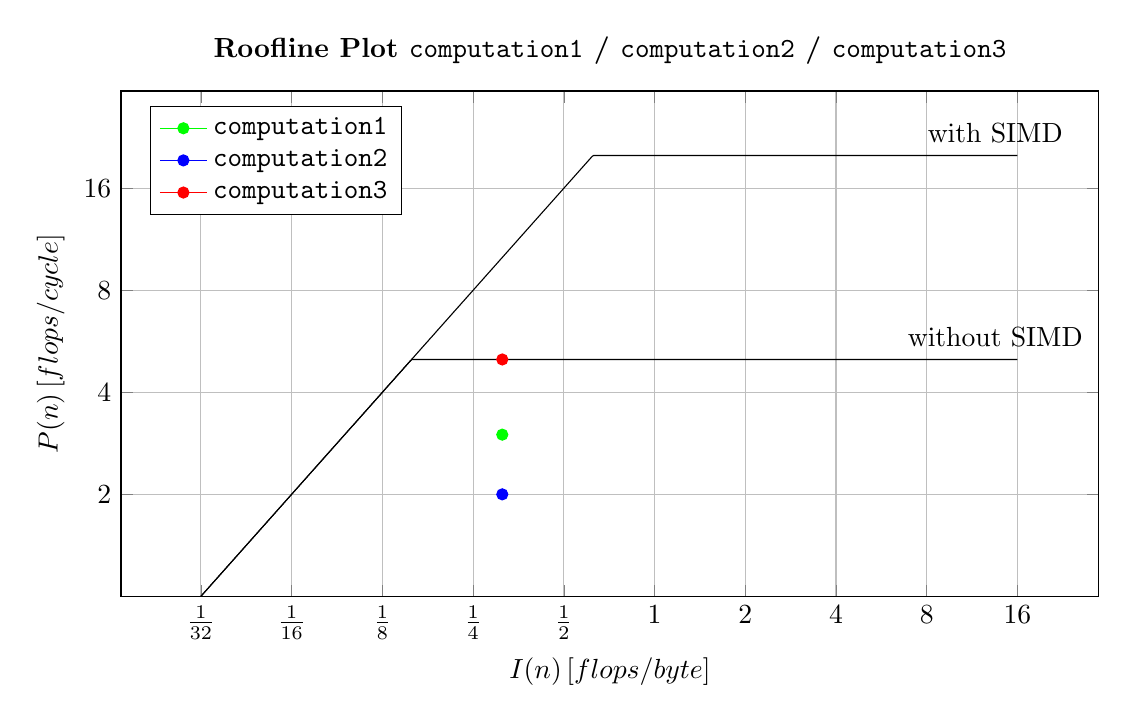
\begin{tikzpicture}
                    \begin{axis}[
                            title=\textbf{Roofline Plot \texttt{computation1} / \texttt{computation2} / \texttt{computation3}},
                            width=14cm,
                            height=8cm,
                            xmode=log,
                            xlabel={$I(n) \, [flops/byte]$},
                            log basis x={2},
                            ylabel=log,
                            ylabel={$P(n) \, [flops/cycle]$},
                            ymode=log,
                            log basis y={2},
                            ymax=31,
                            ymin=1,
                            grid=major,
                            xticklabels={%
                                $0$,
                                $\frac{1}{32}$,
                                $\frac{1}{16}$,
                                $\frac{1}{8}$,
                                $\frac{1}{4}$,
                                $\frac{1}{2}$,
                                $1$,
                                $2$,
                                $4$,
                                $8$,
                                $16$,
                            },
                            yticklabels={
                                $$,
                                $2$,
                                $4$,
                                $8$,
                                $16$,
                            },
                            legend pos=north west,
                    ]
                    % Roofline without SIMD
                    \addplot [
                        black,
                        domain=2^-5:16,
                        samples=500,
                    ] {min(5, 32*x)} [yshift=8pt, xshift=-8pt]
                        node [pos=1] {without SIMD}
                    ;

                    % Roofline with SIMD
                    \addplot [
                        black,
                        domain=2^-5:16,
                        samples=500,
                    ] {min(20, 32*x)} [yshift=8pt, xshift=-8pt]
                        node [pos=1] {with SIMD}
                    ;
                    
                    \addplot[color=green,mark=*] coordinates {(5/16,3)};
                    \addplot[color=blue,mark=*] coordinates {(5/16,2)};
                    \addplot[color=red,mark=*] coordinates {(5/16,5)};
                    \legend{,,\texttt{computation1},\texttt{computation2},\texttt{computation3}} 
                \end{axis}               
                \end{tikzpicture}
                \end{center}
            
            \item When we use vector intrinsics we perform the same number of
                operations and move the same amount of data from main memory
                into cache. Thus, the operational intensity does not change
                when using SIMD instructions. With vector instructions we could 
                potentially get a 4x speedup but the computation gets eventually 
                memory bound.

                If we use SIMD for \verb|computation1| the performance should
                reach $4 \cdot 3 = 12 \, flops/cycle$ but we reach only $10
                \, flops/cycle$ because it is memory bound by the roofline
                model (one can get the bound from the roofline plot). 
                Therefore, \verb|computation1| is \textbf{3.33x} faster
                with SIMD.

                For \verb|computation2| we can reach a performance of $4 \cdot
                2 = 8 \, flops/cycle$ which is not memory bound. Hence, we get
                a full \textbf{4x} speedup for \verb|computation2|.

                \verb|computation3| is also memory bound so we can reach only
                $10 \, flops/cycle$ which gives a speedup of \textbf{2x}. 
            
            \item The modification does not change the number of operations per
                loop iteration so we perform the same 
                amount of work which is still $W(n) = 5n \, flops$ for each
                function.

                If we analyze the strided access pattern we can see that more
                data is moved from memory to the cache. Every iteration we get
                a compulsory miss (sometimes we get none or two misses but the
                average each other out). Each miss moves eight doubles from
                main memory into cache in every iteration so we get
                \begin{equation*}
                    Q(n) \geq 8 \cdot 8 \cdot n = 64n \, bytes
                \end{equation*}
                In all three functions the same access pattern is used and only
                the operations are changed. Thus, we get a new operational
                intensity for all three functions of
                \begin{equation*}
                    I(n) \leq \frac{5n}{64n} = \frac{5}{64} \, flops/byte 
                \end{equation*}

                If we add the new values to the roofline plot we can see that
                the new functions move to the memory bound area of the roofline
                model. The performance bound of \verb|computation2| is still the
                same but we get lower bounds for \verb|computation1| and
                \verb|computation3| because they cannot bring in all required
                data for best performance. Therefore, the new bounds are

                \begin{equation*}
                    P^\prime_1 \leq P^\prime_3 \leq 32 \cdot
                    \frac{5}{64} = 2.5 \, flops/cycle
                \end{equation*}

                We get the following roofline plot where the squares show the
                new bounds. 

                \begin{center}
                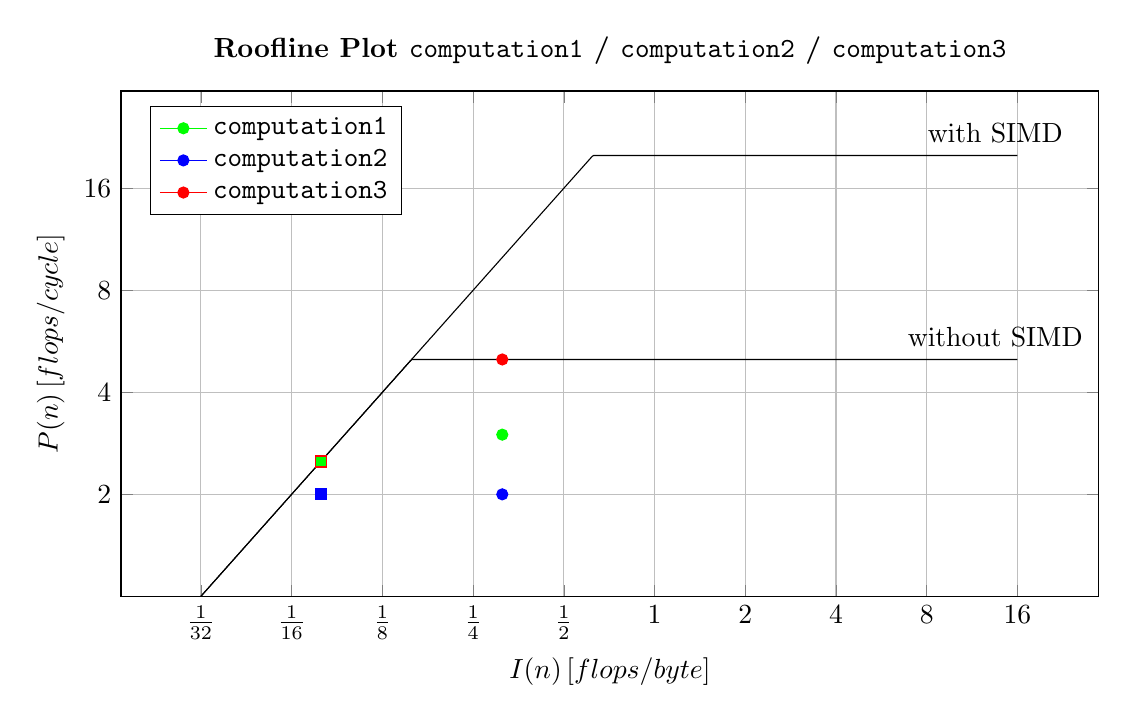
\begin{tikzpicture}
                    \begin{axis}[
                            title=\textbf{Roofline Plot \texttt{computation1} / \texttt{computation2} / \texttt{computation3}},
                            width=14cm,
                            height=8cm,
                            xmode=log,
                            xlabel={$I(n) \, [flops/byte]$},
                            log basis x={2},
                            ylabel=log,
                            ylabel={$P(n) \, [flops/cycle]$},
                            ymode=log,
                            log basis y={2},
                            ymax=31,
                            ymin=1,
                            grid=major,
                            xticklabels={%
                                $0$,
                                $\frac{1}{32}$,
                                $\frac{1}{16}$,
                                $\frac{1}{8}$,
                                $\frac{1}{4}$,
                                $\frac{1}{2}$,
                                $1$,
                                $2$,
                                $4$,
                                $8$,
                                $16$,
                            },
                            yticklabels={
                                $$,
                                $2$,
                                $4$,
                                $8$,
                                $16$,
                            },
                            legend pos=north west,
                    ]
                    % Roofline without SIMD
                    \addplot [
                        black,
                        domain=2^-5:16,
                        samples=500,
                    ] {min(5, 32*x)} [yshift=8pt, xshift=-8pt]
                        node [pos=1] {without SIMD}
                    ;

                    % Roofline with SIMD
                    \addplot [
                        black,
                        domain=2^-5:16,
                        samples=500,
                    ] {min(20, 32*x)} [yshift=8pt, xshift=-8pt]
                        node [pos=1] {with SIMD}
                    ;
                    
                    \addplot[color=green,mark=*] coordinates {(5/16,3)};
                    \addplot[color=green,mark=square*] coordinates {(5/64,2.5)};
                    \addplot[color=blue,mark=*] coordinates {(5/16,2)};
                    \addplot[color=blue,mark=square*] coordinates {(5/64,2)};
                    \addplot[color=red,mark=*] coordinates {(5/16,5)};
                    \addplot[color=red,mark=square] coordinates {(5/64,2.5)};
                    \legend{,,\texttt{computation1},,\texttt{computation2},,\texttt{computation3},} 
                \end{axis}               
                \end{tikzpicture}
                \end{center}
        \end{enumerate}
    \item Skinny Matrix-Matrix Multiplication (15 pts)
    \begin{enumerate}
        \item As everything fits in cache and we have no conflict misses, we
            must transfer each value once from main memory to cache. For $A$ we
            read $m^2$ values, for $B$ we read $mn$ values and for $C$
            we access $2 \cdot mn$ values (considering reads and
            writes). Under the assumption that we have
            a write-back/write-allocate cache and $C$ is only written back at
            the end of the computation, we can bound the I/O cost to
            \begin{equation*}
                Q_a(n,m) = 8m^2 + 8mn + 8 \cdot 2mn = 8m^2 + 24mn \, bytes
            \end{equation*}

        \item When simulating the skinny MMM algorithm one can notice that each
            element of $A$ is read once and $C$ is read and written once to main
            memory (see \textit{Hint}). Thus, the same number of values as
            before is moved between cache and main memory.

            As we can fit only one row of $B$ into cache, we get additional
        conflict misses during the computation. In the function
        \texttt{suboperation\_Ci} we have a miss for every new row of $B$ (as only
        one row fits in cache) so we load $mn$ values in each function call.
        The function \texttt{suboperation\_Ci} gets called 
        $\alpha = \frac{m}{m_c}$ times. We define $M$ as the number of elements
        that fit in cache so $M = n + m_c n + 1$. Therefore, we get a lower
        bound of
        \begin{align*}
        Q(n,m,M) &= 8m^2 + 16mn + 8\alpha m n\\
        &= 8m^2 + 16mn + \frac{8m^2n}{m_c}\\
        &= 9m^2 + 16mn + \frac{8m^2n^2}{M-n-1} & (m_c = \frac{M-n-1}{n})
        \end{align*} 
        \end{enumerate}
\end{enumerate}

\end{document}
